\documentclass[11pt]{article}

\usepackage[margin=1in]{geometry}
\usepackage{amsmath,amssymb}
\usepackage{paralist}
\usepackage{bussproofs}
\newcommand\TernaryInfC[1]{\TrinaryInfC{#1}}

\usepackage{tikz}
\usetikzlibrary{arrows}

\usepackage[noend, ruled]{algorithm2e}
\LinesNumbered
\DontPrintSemicolon

\newcommand{\Z}{\mathbb{Z}}
\newcommand{\eps}{\varepsilon}
\newcommand{\kstar}{^{\textstyle *}}
\newcommand{\kplus}{^+}
\renewcommand{\phi}{\varphi}
\renewcommand{\S}{\mathcal{S}}
\newcommand{\serial}{\gg}
\newcommand{\cserial}{\ggg}
\newcommand{\lift}{\mathsf{lift}}
\newcommand{\inv}{^{-1}}
\newcommand{\incr}{\mathsf{incr}}

\newcommand{\F}{\texttt{F}}
\newcommand{\G}{\texttt{G}}

\begin{document}

\title{COMP 418/518: Homework 3 \\[1ex] \large [Weight of homework: 10\% of the final grade]}
\author{Authors (fill in your names and NetIDs here)}
\date{Due on March 11, 2026 \\ \small (released on February 27, 2026)}

\maketitle

\paragraph{Instructions:}

For this homework, you should work in groups of 3--4 people (i.e., the groups that have been declared and accepted).
%
Only one member of the group should submit on Gradescope.
%
All group members must be included in the submission on the Gradescope system (otherwise no credit will be given).
%
Also specify in your submission file all the members of your group (name and NetID) using the \texttt{\textbackslash authors} macro.
%
The submission must be typed in LaTeX using the provided template.
%
The use of AI systems (including, but not limited to, ChatGPT, Gemini, Copilot, and Claude) is entirely allowed.
%
No discussion or collaboration is allowed outside of the group.
%
Late submissions are not accepted.

\begin{center}
You should provide \emph{pseudocode} for all the algorithms that you describe.
\end{center}

\paragraph{LaTeX Source:}

You must upload the LaTeX source for your submission on Gradescope. Your submission must contain everything that is needed to build the PDF file.

\paragraph{Grading:}

We will give a 5\% grade bonus to students taking COMP 418. The homework will be graded based on correctness, completeness, quality of the solutions, and \textbf{\em quality of writing}.

\paragraph{Guidelines:}

\begin{itemize}
\item
Do not use ellipses in your definitions or your proofs. Instead, use recursive definitions and induction.
\item
Provide a careful justification of every step in your proofs.
\item
If there are logical gaps, unsound mathematical reasoning, false/unclear statements, or any other mistakes, then points will be taken off accordingly.
\item
If a proof is unreadable, then it will receive 0 points. A proof should always be understandable and well written, because the goal is to provide a \emph{convincing} mathematical argument.
\end{itemize}

\paragraph{Notation \& remarks:}

For strings $x, y \in A\kstar$, we say that $x$ is a \emph{prefix} of $y$, and write $x \leq y$, if $xz = y$ for some $z \in A\kstar$. For example, $ab$ is a prefix of $abcde$ because $ab \cdot cde = abcde$. Notice that if $x \leq y$ then there is a \emph{unique} extension $z \in A\kstar$ such that $xz = y$. We write $x\inv y$ to denote this unique extension. For a string $x \in A\kstar$, we write $|x|$ to denote its length. For all strings $x, y \in A\kstar$, it holds that $|x \cdot y| = |x| + |y|$. String concatenation satisfies the following \emph{left cancellation} property: for all $x, y, z \in A\kstar$, $xy = xz$ implies that $y = z$.

For sets $X$ and $Y$, we write $X \to Y$ to denote the set of all functions from $X$ to $Y$.

\clearpage % DO NOT REMOVE THIS
\section*{\fbox{Problem 1 [5 points]}}

Let $A$ be a set. Show that the prefix relation $\leq$ on $A\kstar$ is a partial order (reflexive, antisymmetric and transitive).

\subsection*{Solution for 1}

Fill me in.

\clearpage % DO NOT REMOVE THIS
\section*{\fbox{Problem 2: Denotational Semantics [35 points]}}

In the lecture of February 20 we discussed denotations (functions) of type $A\kplus \to B$ and of type $A\kplus \to B\kplus$. Recall that a function $f: A\kplus \to B$ describes a streaming computation in the following way: for an input history $x \in A\kplus$, the value $f(x)$ is the last output item after consuming $x$. We call $f$ an \emph{incremental} denotation, because it gives us the output increment. A function $\phi: A\kplus \to B\kplus$ can sometimes describe a streaming computation in the following way: for an input history $x \in A\kplus$, the value $\phi(x)$ is the overall output history after consuming $x$. We call $\phi$ a \emph{cumulative} denotation, because it gives us the cumulative (overall) output.

\textbf{\em Remark}: In this problem, we are only concerned with streaming computations that (i) produce exactly one output item per step (i.e., for each input item), and (ii) do \emph{not} produce any output at the very beginning (i.e., before the first input item is seen).

\subsection*{\underline{Part 2A} [5 points]}

Define an injective function $\lift$ from the set $A\kplus \to B$ to the set $A\kplus \to B\kplus$. That is, $\lift: (A\kplus \to B) \to (A\kplus \to B\kplus)$ and $\lift$ is injective. The function $\lift$ should convert an incremental denotation to a cumulative denotation. Provide a proof that $\lift$ is injective.

\subsubsection*{Solution for 2A}

Fill me in.

\subsection*{{\underline{Part 2B} [15 points]}}

For all sets $A$ and $B$, specify a subset $\S(A,B) \subseteq (A\kplus \to B\kplus)$ so that $\lift$ is a one-to-one correspondence (bijection) from $A\kplus \to B$ to $\S(A,B)$. Provide a proof that $\lift$ is a bijection.

\subsubsection*{Solution for 2B}

Fill me in.

\subsection*{\underline{Part 2C} [15 points]}

Recall the operation $\serial$ (serial composition) on incremental denotations from the lecture of February 20. Below is a description of how $\serial$ is applied to ensure that the types match up appropriately:
\[
  \AxiomC{$f: A\kplus \to B$}
  \AxiomC{$g: B\kplus \to C$}
  \BinaryInfC{$f \serial g: A\kplus \to C$}
  \DisplayProof
\]
The above notation is sometimes referred to as a \emph{type rule} in the context of programming languages.
\begin{enumerate}[(1)]
\item
Define a corresponding operation $\cserial$ (serial composition)\footnote{We use the notation $\cserial$ to differentiate more easily with serial composition on incremental denotations.} on cumulative denotations with the following type rule:
\[
  \AxiomC{$\phi: A\kplus \to B\kplus$}
  \AxiomC{$\psi: B\kplus \to C\kplus$}
  \BinaryInfC{$\phi \cserial \psi: A\kplus \to C\kplus$}
  \DisplayProof
\]
\item
Show that $\phi \cserial \psi \in \S(A,C)$ whenever $\phi \in \S(A,B)$ and $\psi \in \S(B,C)$.
\item
Moreover, show that
$
  \lift(f \serial g) =
  \lift(f) \cserial \lift(g)
$
for all $f: A\kplus \to B$ and $g: B\kplus \to C$.
\end{enumerate}

\subsubsection*{Solution for 2C}

Fill me in.

\clearpage % DO NOT REMOVE THIS
\section*{\fbox{Problem 3: Pipeline Fusion [60 points]}}

Assume that we have the same (restricted) programming model for streaming computations that we considered in Problem 2.

\subsection*{\underline{Part 3A} [4 points]}

Consider the incremental denotation $f: \Z\kplus \to \Z$, defined by $f(x) = x$ and $f(u x y) = y - x$ for every $u \in \Z\kstar$ and $x, y \in \Z$. Give a description in English of the computation that $f$ describes and provide an implementation using pseudocode. Is your implementation stateful or stateless?

\subsubsection*{Solution for 3A}

The denotation $f$ computes the discrete first difference of the input stream, with a special case at the first step:
\[
\forall x \in \Z,\ f(x)=x
\quad\text{and}\quad
\forall u \in \Z\kstar,\ \forall x,y \in \Z,\ f(u x y)=y-x.
\]
So the output is the current value minus the previous value (except at the first item, where the output is the item itself). The implementation is \emph{stateful}, because it must remember the previous input item.
\begin{center}
\begin{minipage}{0.3\textwidth}
\SetAlgoLined
\setcounter{AlgoLine}{0}

\tcp{Implementation of $f$}

\tcp{State:}

$\textit{hasPrev} \in \{\texttt{false}, \texttt{true}\}$, initially \texttt{false}

$\textit{prev} \in \Z$ (value irrelevant while $\textit{hasPrev}=\texttt{false}$)

\SetKwFunction{Update}{Update}
\SetKwProg{Fn}{Function}{:}{end}
\Fn{\Update{$\Z\ x$}}{
	\If(\tcp*[f]{first input item}){$\textit{hasPrev}=\texttt{false}$}{
		$\textit{hasPrev} \leftarrow \texttt{true}$

		$\textit{prev} \leftarrow x$

		\Return $x$
	}
	$\Z\ \textit{out} \leftarrow x-\textit{prev}$

	$\textit{prev} \leftarrow x$

	\Return $\textit{out}$
}
\end{minipage}
\end{center}

\subsection*{\underline{Part 3B} [3 points]}

Consider the incremental denotation $g: \Z\kplus \to \Z$, defined by $g(x) = x$ and $g(u x) = g(u) + x$ for every $u \in \Z\kplus$ and $x \in \Z$. Give a description in English of the computation that $g$ describes and provide an implementation using pseudocode. Is your implementation stateful or stateless?

\subsubsection*{Solution for 3B}

The denotation $g$ computes the running prefix sum of the input stream:
\[
\forall x \in \Z,\ g(x)=x
\quad\text{and}\quad
\forall u \in \Z\kplus,\ \forall x \in \Z,\ g(u x)=g(u)+x.
\]
So at each step, the output is the total sum of all items seen so far. The implementation is \emph{stateful}, because it must remember the running sum.
\begin{center}
\begin{minipage}{0.3\textwidth}
\SetAlgoLined
\setcounter{AlgoLine}{0}

\tcp{Implementation of $g$}

\tcp{State:}

$\Z\ \textit{sum}$, initially $0$

\SetKwFunction{Update}{Update}
\SetKwProg{Fn}{Function}{:}{end}
\Fn{\Update{$\Z\ y$}}{
	$\textit{sum} \leftarrow \textit{sum} + y$

	\Return $\textit{sum}$
}
\end{minipage}
\end{center}

\subsection*{\underline{Part 3C} [8 points]}

Let $\F$ be your implementation of $f$ (from Part 3A) and $\G$ be your implementation of $g$ (from Part 3B). Provide a single streaming algorithm that simulates the execution of the following pipeline:
\begin{center}
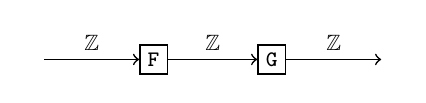
\begin{tikzpicture}[->, >=to, auto, node distance=1.5cm, semithick, transform shape]
%
\footnotesize
%
\node (M1) {};
\node (M2) [draw, right of=M1] {\F};
\node (M3) [draw, right of=M2] {\G};
\node (M4) [right of=M3] {};
%
\path (M1) edge node {$\Z$} (M2);
\path (M2) edge node {$\Z$} (M3);
\path (M3) edge node {$\Z$} (M4);
\end{tikzpicture}
\end{center}
Use the ``fusion'' construction what we discussed on February 18. How many arithmetic operations does your implementation perform per step (i.e., for every input data item)?

\subsubsection*{Solution for 3C}

Using fusion, we combine the state of $\F$ and $\G$ into one machine state. The fused state is the product of the two states:
\[
(\textit{hasPrev},\textit{prev}) \text{ for } \F
\quad\text{and}\quad
\textit{sum} \text{ for } \G.
\]
On each step we first compute the output of $\F$, then use it to update $\G$.
\begin{center}
\begin{minipage}{0.3\textwidth}
\SetAlgoLined
\setcounter{AlgoLine}{0}

\tcp{Pipeline(\F, \G)}

\tcp{State:}

$\textit{hasPrev} \in \{\texttt{false}, \texttt{true}\}$, initially \texttt{false}

$\textit{prev} \in \Z$ (value irrelevant while $\textit{hasPrev}=\texttt{false}$)

$\Z\ \textit{sum}$, initially $0$

\SetKwFunction{Update}{Update}
\SetKwProg{Fn}{Function}{:}{end}
\Fn{\Update{$\Z\ x$}}{
	\If{$\textit{hasPrev}=\texttt{false}$}{
		$\textit{hasPrev} \leftarrow \texttt{true}$

		$\textit{prev} \leftarrow x$

		$\Z\ d \leftarrow x$
	}
	\Else{
		$\Z\ d \leftarrow x-\textit{prev}$

		$\textit{prev} \leftarrow x$
	}
	$\textit{sum} \leftarrow \textit{sum}+d$

	\Return $\textit{sum}$
}
\end{minipage}
\end{center}

This fused implementation performs one subtraction and one addition on every step after the first step. At the first step, it performs one addition. Therefore the worst-case number of arithmetic operations per step is $2$.

\subsection*{\underline{Part 3D} [15 points]}

The implementation ``\texttt{Pipeline(\F, \G)}'' that you provided in Part 3C is one out of many streaming algorithms that compute the incremental denotation $f \serial g: \Z\kplus \to \Z$. Is it possible to provide a more efficient implementation of $f \serial g$ (i.e., one that uses less memory and performs fewer operations per step)? If your answer is ``yes'', provide the most efficient implementation you can think of and justify its correctness.

\subsubsection*{Solution for 3D}

Yes. A strictly more efficient implementation exists.

Let the input history have length $n$, and let $x_i$ denote the $i$-th input item. Define $d_i$ as the $i$-th output of $\F$:
\[
d_1=x_1
\quad\text{and}\quad
d_i=x_i-x_{i-1}\ \text{for all integers}\ i\ \text{with}\ 2\le i\le n.
\]
Then the output of $\G$ at step $n$ is
\[
\sum_{i=1}^{n}d_i
=
x_1+\sum_{i=2}^{n}(x_i-x_{i-1})
=x_n.
\]
So for every history of length $n$, the value of $f \serial g$ is the last input item $x_n$. This is exactly the identity incremental denotation on $\Z\kplus$.

Hence an optimal implementation is:
\[
\texttt{Update}(x)\ \texttt{return}\ x.
\]
This implementation is stateless, uses less memory than \texttt{Pipeline(\F,\G)}, and performs zero arithmetic operations per step.

\subsection*{\underline{Part 3E} [30 points]}

Let $\F$ be your implementation of $f$ (from Part 3A) and $\G$ be your implementation of $g$ (from Part 3B). Suppose that $P$ is a pipeline in which every stage is either $\F$ or $\G$ and there are $k \geq 0$ more $\G$ stages than $\F$ stages. For example, the pipeline
\begin{center}
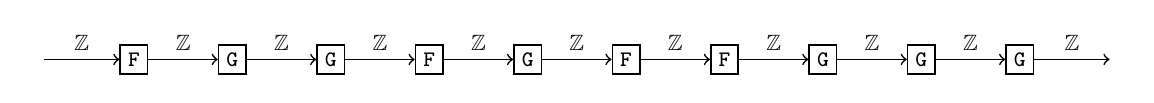
\begin{tikzpicture}[->, >=to, auto, node distance=1.25cm, semithick, transform shape]
%
\footnotesize
%
\node (M1) {};
\node (M2) [draw, right of=M1] {\F};
\node (M3) [draw, right of=M2] {\G};
\node (M4) [draw, right of=M3] {\G};
\node (M5) [draw, right of=M4] {\F};
\node (M6) [draw, right of=M5] {\G};
\node (M7) [draw, right of=M6] {\F};
\node (M8) [draw, right of=M7] {\F};
\node (M9) [draw, right of=M8] {\G};
\node (M10) [draw, right of=M9] {\G};
\node (M11) [draw, right of=M10] {\G};
\node (M12) [right of=M11] {};
%
\path (M1) edge node {$\Z$} (M2);
\path (M2) edge node {$\Z$} (M3);
\path (M3) edge node {$\Z$} (M4);
\path (M4) edge node {$\Z$} (M5);
\path (M5) edge node {$\Z$} (M6);
\path (M6) edge node {$\Z$} (M7);
\path (M7) edge node {$\Z$} (M8);
\path (M8) edge node {$\Z$} (M9);
\path (M9) edge node {$\Z$} (M10);
\path (M10) edge node {$\Z$} (M11);
\path (M11) edge node {$\Z$} (M12);
\end{tikzpicture}
\end{center}
has 6 $\G$ stages and 4 $\F$ stages, which means that $k = 2$. Provide an efficient implementation of the same computation that $P$ performs. You can use $k \geq 0$ as a parameter in your implementation. Justify the correctness of your implementation.

\subsubsection*{Solution for 3E}

Let $\mathbf{id}: \Z\kplus \to \Z$ be the identity incremental denotation, $\mathbf{id}(u x)=x$.

From Part 3D and the symmetric calculation, we have both cancellation laws:
\[
f \serial g = \mathbf{id}
\quad\text{and}\quad
g \serial f = \mathbf{id}.
\]
Consider any pipeline word over $\{\F,\G\}$. Repeatedly delete adjacent pairs $\F\G$ or $\G\F$. Each deletion preserves denotation (by the equalities above) and shortens the word by $2$, so the process terminates. The remaining reduced word has no adjacent opposite symbols. Since the alphabet has only two symbols, the reduced word must be either $\F^m$ or $\G^m$ for some $m \ge 0$. Because the original pipeline has $k \ge 0$ more $\G$ stages than $\F$ stages, the reduced form is $\G^k$. Therefore, $P$ is equivalent to $k$ serial copies of $\G$.

So we only need an implementation for $\G^k$.
\begin{center}
\begin{minipage}{0.3\textwidth}
\SetAlgoLined
\setcounter{AlgoLine}{0}

\tcp{Pipeline $P$ with $k \geq 0$}

\tcp{State:}

Array $S$ indexed by integers $i$ with $1 \le i \le k$

\For{$i \leftarrow 1$ \KwTo $k$}{
	$S[i] \leftarrow 0$
}

\SetKwFunction{Update}{Update}
\SetKwProg{Fn}{Function}{:}{end}
\Fn{\Update{$\Z\ x$}}{
	\If{$k=0$}{
		\Return $x$
	}
	$S[1] \leftarrow S[1] + x$

	\For{$i \leftarrow 2$ \KwTo $k$}{
		$S[i] \leftarrow S[i] + S[i-1]$
	}
	\Return $S[k]$
}
\end{minipage}
\end{center}

\textbf{Correctness of the implementation.}
For each integer $i$ with $1 \le i \le k$, let $G_i(n)$ be the output of the $i$-th $\G$ stage at step $n$ in a pipeline of $k$ $\G$ stages. Also set $G_0(n)=x_n$. The stage recurrence is
\[
G_i(n)=G_i(n-1)+G_{i-1}(n), \quad G_i(0)=0.
\]
The algorithm maintains the invariant $S[i]=G_i(n)$ after processing step $n$.

Base case ($n=1$): after one update, $S[1]=x_1=G_1(1)$, and then each loop update gives $S[i]=S[i]+S[i-1]=0+G_{i-1}(1)=G_i(1)$.

Induction step: assume after step $n-1$, $S[i]=G_i(n-1)$ for all $i$. At step $n$, the update for $S[1]$ yields
\[
S[1]\leftarrow S[1]+x_n=G_1(n-1)+G_0(n)=G_1(n).
\]
Then for each $i\ge 2$, after $S[i-1]$ has been updated to $G_{i-1}(n)$,
\[
S[i]\leftarrow S[i]+S[i-1]=G_i(n-1)+G_{i-1}(n)=G_i(n).
\]
Thus the invariant holds for step $n$. Therefore, after every step, the returned value $S[k]$ equals the output of $\G^k$, which equals the output of pipeline $P$.

The implementation uses $k$ integer state variables and performs exactly $k$ additions per step when $k>0$ (and zero additions when $k=0$).


\bibliographystyle{plain}

\end{document}
